\begin{figure}[H]
\centering
\shorthandoff{<>}
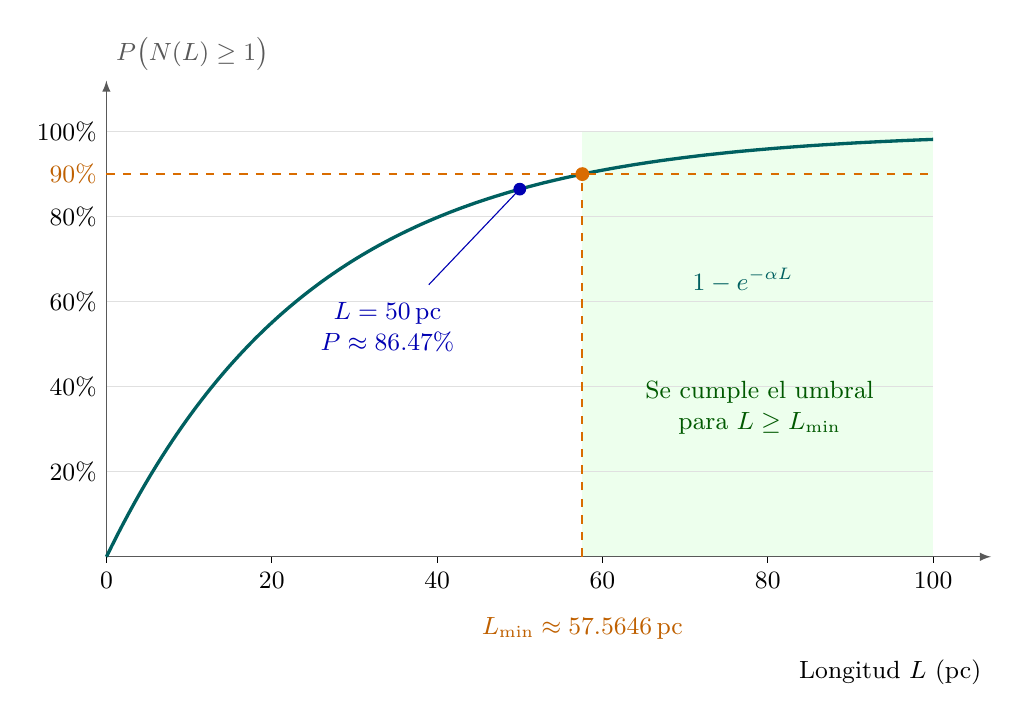
\begin{tikzpicture}[x=0.105cm,y=5.4cm,font=\small,>=latex]
  \fill[green!7] (57.5646,0) rectangle (100,1);
  \foreach \level/\percentage in {0.2/20,0.4/40,0.6/60,0.8/80,1/100}{
    \draw[black!12] (0,\level) -- (100,\level);
    \node[left] at (0,\level) {$\percentage\%$};
  }
  \draw[->,black!65] (0,0) -- (107,0);
  \draw[->,black!65] (0,0) -- (0,1.12)
    node[above right] {$P\bigl(N(L)\ge1\bigr)$};
  \draw[teal!75!black,very thick] plot[domain=0:100,samples=150,variable=\lengthvalue]
    ({\lengthvalue},{1-exp(-0.04*\lengthvalue)});
  \draw[dashed,orange!85!black,thick] (0,0.9) -- (100,0.9);
  \node[left,text=orange!75!black] at (0,0.9) {$90\%$};
  \draw[dashed,orange!85!black,thick] (57.5646,0) -- (57.5646,0.9);
  \fill[orange!85!black] (57.5646,0.9) circle (2.5pt);
  \fill[blue!70!black] (50,0.864665) circle (2.3pt);
  \draw[blue!70!black,thin] (50,0.864665) -- (39,0.64);
  \node[align=center,text=blue!70!black] at (34,0.54)
    {$L=50\,\mathrm{pc}$\\$P\approx86.47\%$};
  \node[align=center,text=green!35!black] at (79,0.35)
    {Se cumple el umbral\\para $L\ge L_{\min}$};
  \node[text=teal!75!black] at (77,0.65) {$1-e^{-\alpha L}$};
  \foreach \tick in {0,20,40,60,80,100}{
    \draw (\tick,0) -- (\tick,-0.015) node[below] {$\tick$};
  }
  \node[anchor=north,text=orange!75!black] at (57.5646,-0.12)
    {$L_{\min}\approx57.5646\,\mathrm{pc}$};
  \node[anchor=north east] at (107,-0.22) {Longitud $L$ (pc)};
\end{tikzpicture}
\shorthandon{<>}
\caption{Probabilidad de encontrar al menos una estrella en función de la longitud observada, con $\alpha=0.04\,\mathrm{pc}^{-1}$. El cruce con el nivel del $90\%$ determina $L_{\min}=25\ln 10\,\mathrm{pc}$. La zona verde señala las longitudes que satisfacen el requisito. Esta probabilidad se aproxima a $1$ sin crecer linealmente, a diferencia del número esperado $E[N(L)]=\alpha L$.}
\label{fig:poisson-longitud}
\end{figure}